\chapter{Results}

In this chapter, we present the findings of our research, which aims to evaluate the impact of the COVID-19 pandemic on supply chain resilience for perishable goods through a mixed-methods approach. This chapter is organized into three main parts to systematically address our research objectives. First, we will present the results derived from the Partial Least Squares Structural Equation Modeling (PLS-SEM) analysis. This quantitative analysis was conducted using survey data to examine the relationships between key constructs such as pandemic disruption, change management, and resilience effectiveness. The PLS-SEM results will provide insights into the statistical validity of these constructs and the strength and significance of the paths hypothesized in our model. Following the quantitative analysis, we will delve into the findings from the qualitative analysis of the long-form interview conducted with a supply chain professional. This section will explore the experiential insights shared by the interviewee, shedding light on the practical challenges faced by suppliers of perishable goods during the pandemic, the strategies adopted to enhance supply chain resilience, and the perceived effectiveness of these strategies. The qualitative results will complement the quantitative findings by providing a nuanced understanding of the context and the real-world applications of the theoretical constructs examined in the PLS-SEM analysis.

After presenting the individual results from both analyses, we will synthesize the findings to provide a holistic view of the study. This synthesis will enable us to draw connections between the quantitative data and qualitative insights, thereby answering our primary research questions concerning the resilience of supply chains for perishable goods during the COVID-19 pandemic. Finally, we will evaluate the validity of our hypotheses based on the combined evidence, determining which hypotheses are supported or refuted by the research findings. This comprehensive approach will help us identify key strategies and challenges in developing resilient supply chains and provide recommendations for future preparedness against similar disruptions.

\section{Results of PLS-SEM}

\begin{figure}[ht]
  \centering
  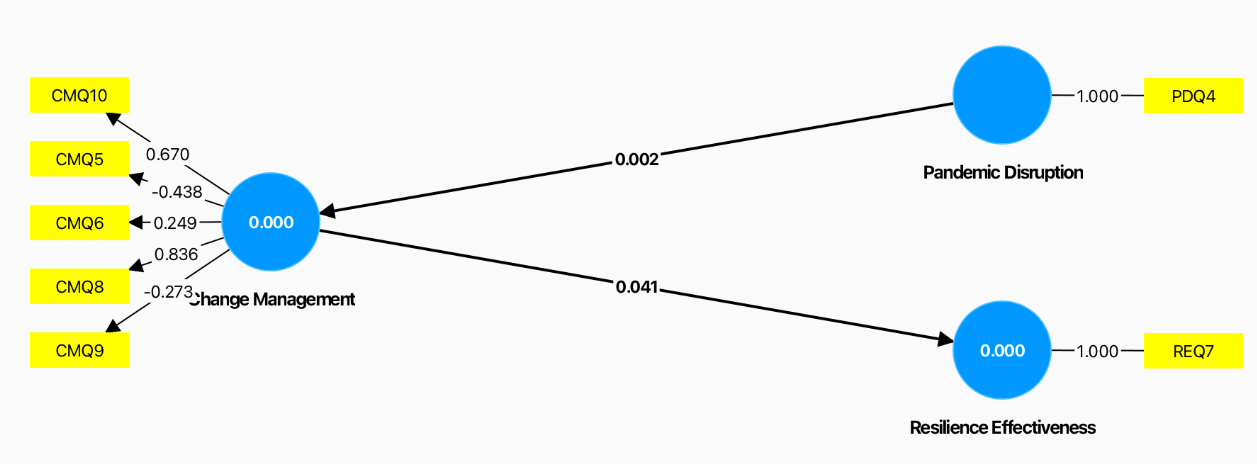
\includegraphics[width=1\textwidth]{figure/pls_sem_results_cropped.png}
  \caption{PLS-SEM Results showcasing path coefficients between constructs.}
  \label{fig:pls_sem_results}
\end{figure}

The results of our PLS-SEM analysis, depicted in Figure \ref{fig:pls_sem_results}, reveal the path coefficients among the constructs of Pandemic Disruption, Change Management, and Resilience Effectiveness. The path coefficient from Pandemic Disruption to Change Management is 0.002, suggesting a minimal positive influence of pandemic-induced disruptions on the extent of change management strategies implemented. This indicates that while pandemic disruptions might necessitate some strategic changes, the direct impact observed here is negligible. Conversely, the path coefficient from Resilience Effectiveness to Change Management is 0.041, implying a slight positive relationship. This suggests that as the effectiveness of resilience strategies increases, there is a marginal but positive impact on change management practices, indicating that companies with effective resilience strategies may still engage in proactive change management. 

The negative coefficients observed within the Change Management construct, such as -0.438 for CMQ5, -0.249 for CMQ6, and -0.273 for CMQ9, indicate that these specific aspects of change management may inversely relate to the overall construct. This could mean that certain change management practices, possibly those perceived as less effective or unnecessary, might detract from the overall strategic change efforts. The positive coefficients, such as 0.670 for CMQ10 and 0.836 for CMQ8, highlight the aspects that contribute positively to Change Management, signifying effective practices that enhance strategic adaptability. The significant values of 1.000 for PDQ4 and REQ7 indicate strong relationships of these specific questions with their respective constructs, emphasizing their reliability as indicators. Following the discussion on the path coefficients and their implications, we now turn our attention to additional metrics and validity assessments to provide further analysis of the model's performance.

\begin{figure}[ht]
  \centering
  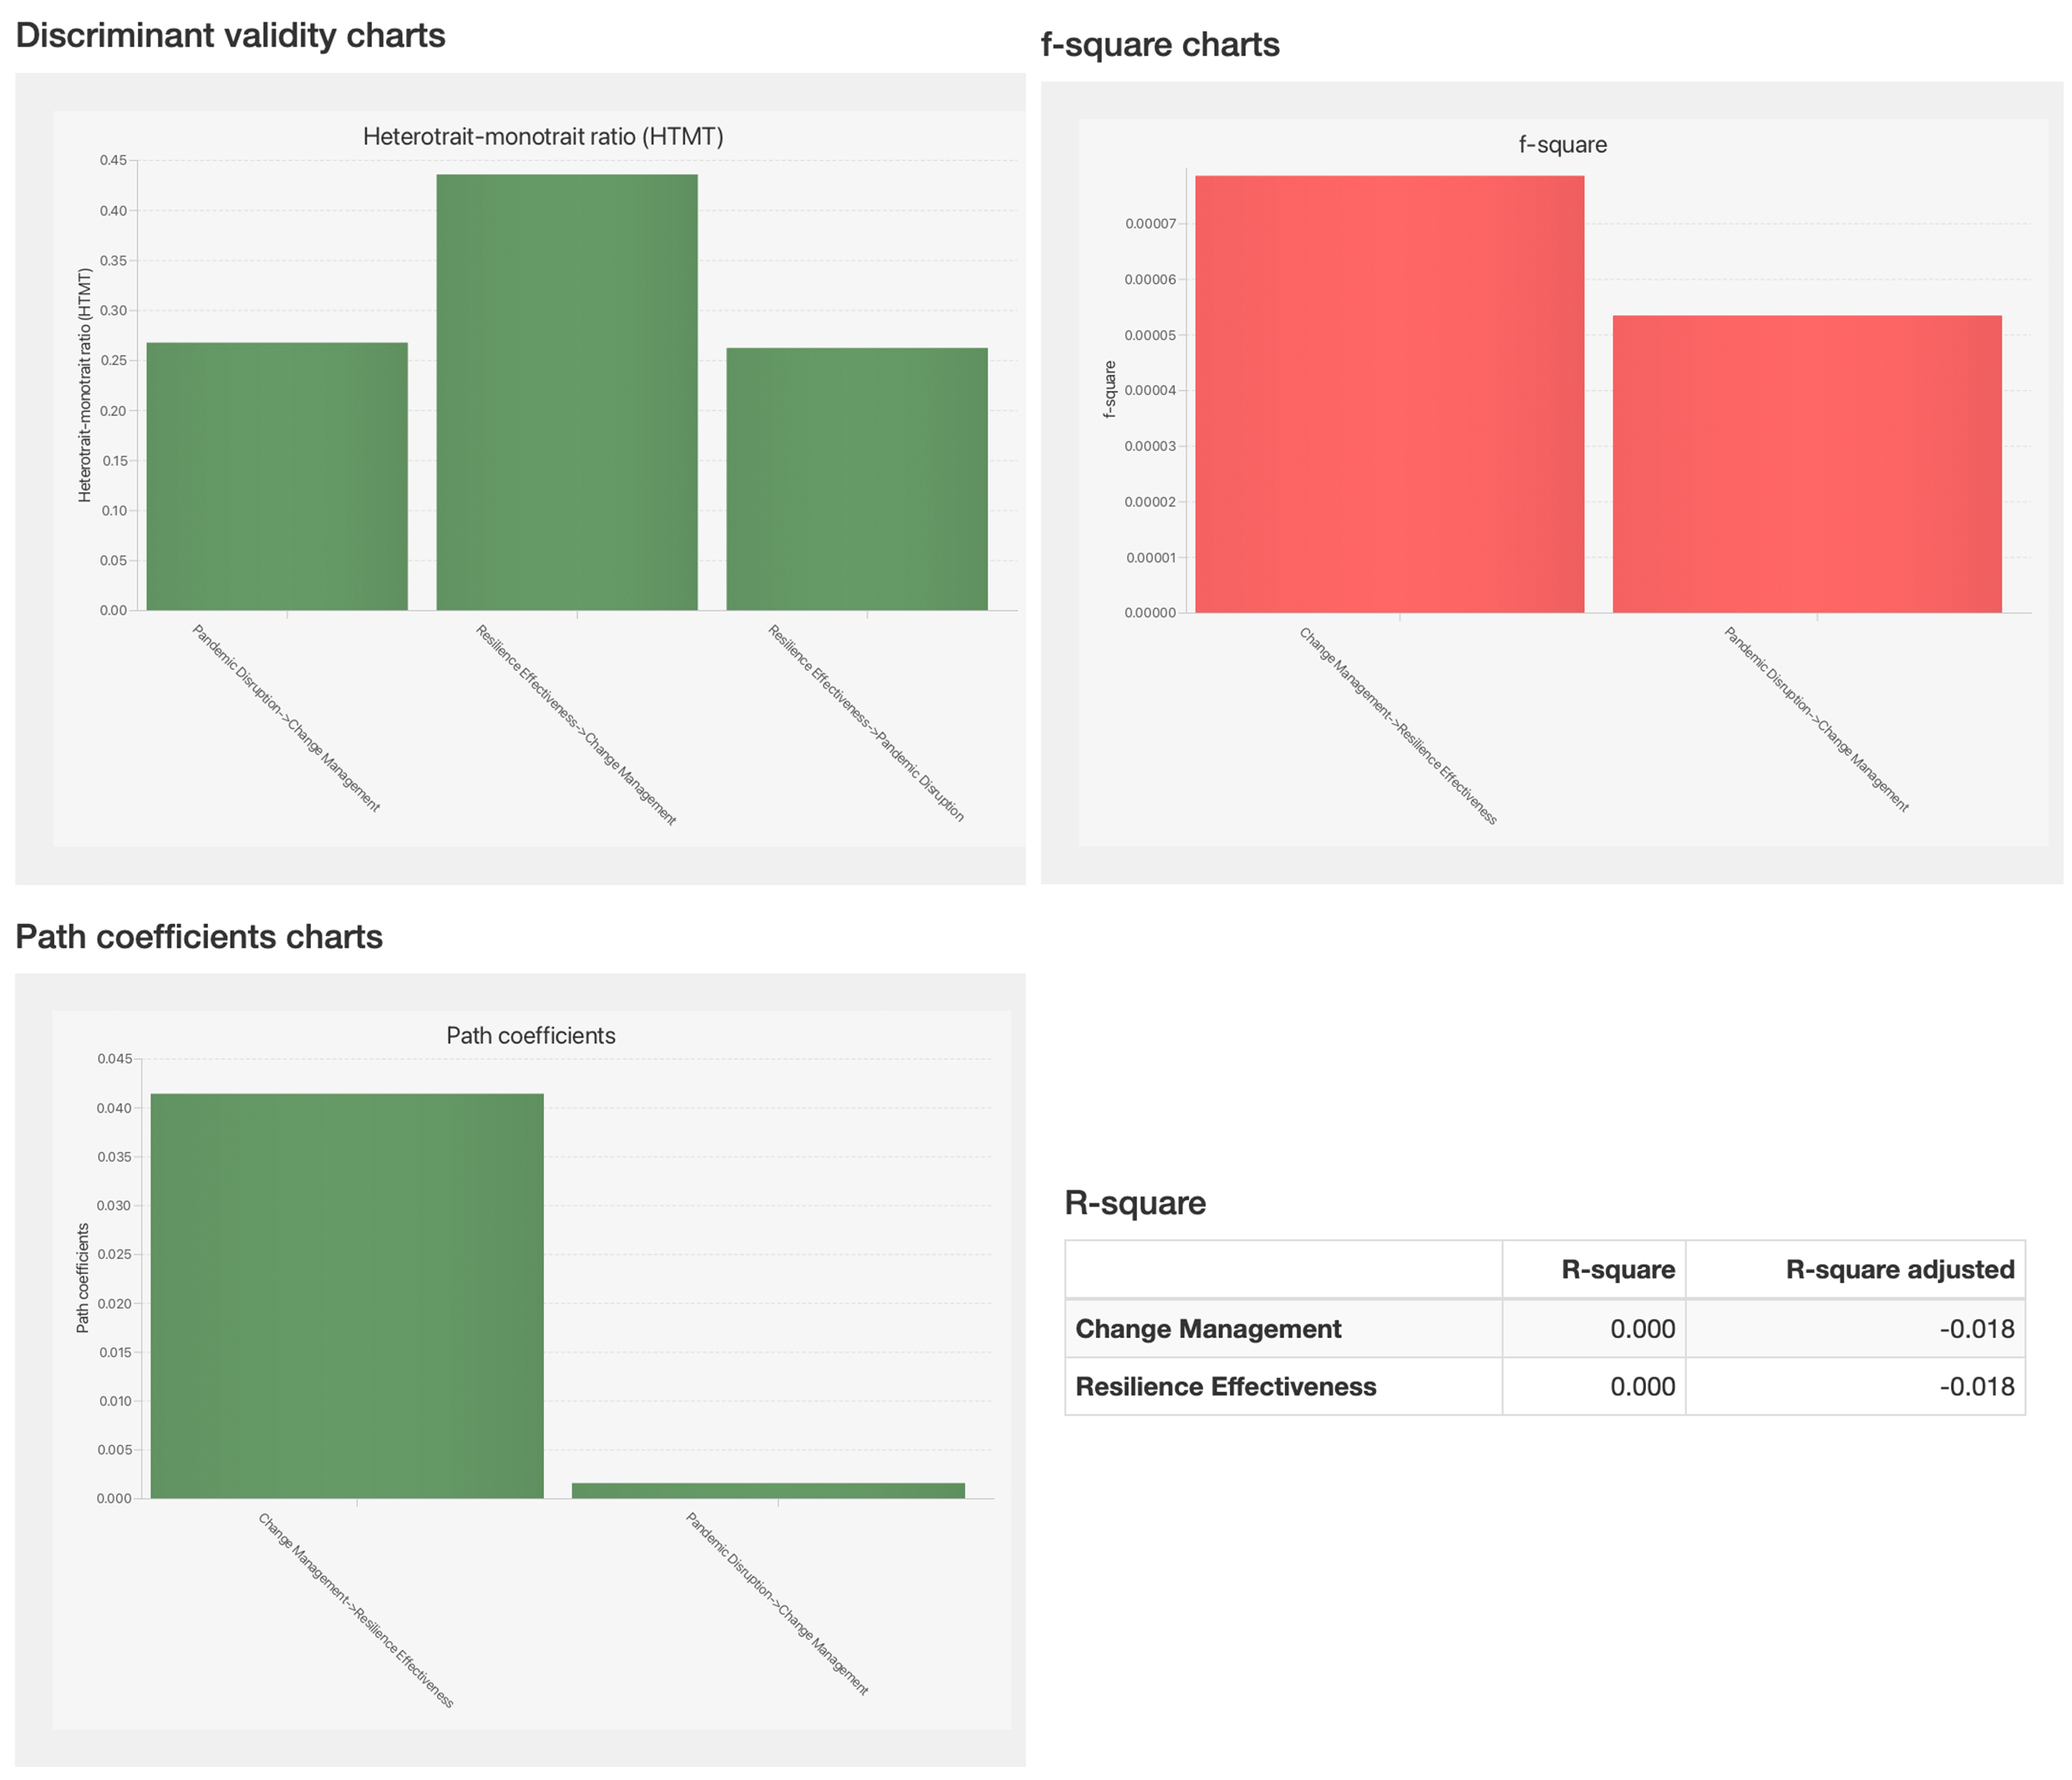
\includegraphics[width=1\textwidth]{figure/other_results.png}
  \caption{Other statistics from PLS-SEM analysis.}
  \label{fig:other_results}
\end{figure}

The results and analysis of PLS-SEM, as depicted in Figure \ref{fig:other_results}, offer further understanding of the relationships between the constructs of Pandemic Disruption, Change Management, and Resilience Effectiveness. The path coefficients chart confirms the previously discussed minimal impact, with the coefficient from Pandemic Disruption to Change Management being virtually zero (0.002), indicating a negligible direct effect. The slightly positive coefficient from Resilience Effectiveness to Change Management (0.041) suggests a weak but positive influence, implying that effective resilience strategies marginally contribute to change management efforts. The R-square values for both Change Management and Resilience Effectiveness are zero, indicating that the model does not explain any variance in these constructs, which may suggest either the lack of a strong relationship or limitations in the model's ability to capture the dynamics. 

The f-square values, though small, provide insight into the effect sizes, with Change Management to Resilience Effectiveness showing a slightly higher value compared to Pandemic Disruption to Change Management, indicating that resilience strategies have a somewhat more substantial influence on change management. The discriminant validity, assessed through the Heterotrait-Monotrait ratio (HTMT), indicates acceptable values below the threshold of 0.85, confirming that the constructs are distinct from each other. The SRMR values are 0.172 for the saturated model and 0.180 for the estimated model, both exceeding the recommended threshold of 0.08, suggesting a poor model fit and potential issues with the structural model specification. These results imply that while some relationships are weakly supported, the overall model does not adequately capture the variance and relationships between the constructs, indicating the need for model refinement or consideration of additional variables to better understand the dynamics at play.

Based on analysis and observation of our dataset, several factors have been identified that may explain why we were unable to establish strong correlations in our PLS-SEM analysis. Firstly, the lack of variability in the Change Management questions (CMQ5, CMQ6, CMQ8, CMQ9, CMQ10), where responses were predominantly '1' (Yes), significantly limits the statistical power of our analysis. The homogeneity in these responses means there is insufficient variation to explain the variance in dependent constructs, thereby hindering the detection of meaningful relationships. While the Pandemic Disruption variable (PDQ4) exhibited more variability, ranging from 0.8 to 5, its effectiveness in revealing correlations is compromised when paired with less variable indicators. Similarly, Resilience Effectiveness (REQ7) showed reasonable variability, ranging from 1.5 to 5, but the overall analysis suffers from the lack of diversity in binary responses. 

The binary nature and the high prevalence of a single response category diminish the ability of PLS-SEM to uncover underlying patterns, as significant paths are often established through variance explained by independent variables. The presence of potential ceiling effects, where binary indicators in the Change Management construct consistently hit the upper limit of their scale, further complicates the analysis by obscuring genuine relationships. This effect results in insufficient differentiation among responses, making it difficult to discern how changes in one variable relate to another. Lastly, the model configuration and theoretical considerations play a crucial role; our current model setup may not adequately capture the expected relationships if the theoretical assumptions are not perfectly aligned with the observed data. 

The predominance of 'yes' responses in the Change Management questions indicates that minor deviations might not statistically explain variations in Resilience Effectiveness, especially if the resilience question encompasses broader aspects of the pandemic's impact than anticipated. Consequently, while the results might indicate no correlation, it is also possible that due to the dataset's characteristics, existing correlations could not be established, highlighting the need for further refinement and consideration of additional variables.


\section{Results from the Interview}

Based on the detailed analysis of the interview, the evidence strongly supports Hypothesis 1, which asserts that suppliers of perishable goods faced significant disruptions in their supply chains due to the COVID-19 pandemic. The interview highlighted multiple challenges such as supply shortages, transportation delays, and the need for rapid adjustments in inventory strategies. These findings align with the notion that the pandemic caused substantial disruptions across various supply chain components. For example, external events like the blockage of the Suez Canal created severe transportation delays, leading to bottlenecks and increased complexity in demand forecasting. Such incidents underscore the vulnerability of supply chains to sudden disruptions and emphasize the necessity for flexibility in managing these challenges. Additionally, managing transportation delays and shortages required frequent recalibration of logistics and inventory management strategies, further validating Hypothesis 1. Although the interview did not directly address labor constraints, it implied that disruptions in material availability and workforce management were significant challenges, contributing to higher operational costs and supply chain instability. Conversely, there is little to no evidence supporting Hypothesis 2, which posits that suppliers of perishable goods did not experience substantial disruptions. The cumulative evidence clearly points to a broad range of disruptions affecting both upstream and downstream supply chain activities.

Thus, the evaluation concludes that Hypothesis 1 is substantiated by the evidence presented in the interview. The interviewee's account of the supply chain challenges faced during the pandemic confirms that the disruptions were significant, widespread, and necessitated substantial adjustments to supply chain strategies and practices.

In evaluating Hypothesis 2, which suggests that suppliers of perishable goods have implemented new strategies and procedures to enhance resilience and preparedness, the evidence from the interview is compelling. The interview highlighted various immediate and long-term strategies that companies adopted in response to the pandemic, such as local warehousing, diversification of suppliers, and increased collaboration with both large and small suppliers. These strategies reflect a proactive approach aimed at strengthening supply chain resilience and preparing for future disruptions. Further support for Hypothesis 2 is found in the long-term strategic changes adopted by companies, including the adoption of technology for real-time data sharing and enhanced visibility across the supply chain. The establishment of crisis management teams and the formation of new supplier partnerships also demonstrate a commitment to improving preparedness for future crises. These actions illustrate a strategic shift towards more resilient and flexible supply chains, aligning with the hypothesis that companies have made significant efforts to enhance their resilience. Conversely, evidence contradicts the notion that companies have not implemented significant changes or strategies to enhance supply chain resilience. The findings show that companies have actively pursued various strategic responses to address the pandemic's challenges. The use of technology, creation of crisis management teams, and emphasis on continuous evaluation of supplier networks all point to deliberate efforts to improve supply chain robustness.

In summary, the evidence from the interview strongly supports Hypothesis 1 and Hypothesis 2, demonstrating significant disruptions during the pandemic and the implementation of new strategies to enhance supply chain resilience.

\section{Integrated Results and Analysis}

In this section, we synthesize the findings from the PLS-SEM analysis and the long-form interviews to provide a comprehensive understanding of the impact of the COVID-19 pandemic on supply chain resilience for perishable goods. Finally we attempt to answer the Research Questions and validate or invalidate the Hypothesis.

The PLS-SEM analysis revealed insights into the relationships between key constructs: Pandemic Disruption, Change Management, and Resilience Effectiveness. The path coefficients indicated minimal direct impact from Pandemic Disruption to Change Management (0.002), suggesting that while the pandemic led to some adjustments, the changes in management practices were not significantly influenced by the disruptions. Conversely, the slight positive relationship from Resilience Effectiveness to Change Management (0.041) implied that effective resilience strategies marginally contributed to improvements in change management practices. However, the overall model did not explain much variance in the constructs, as evidenced by the R-square values of zero and the high SRMR values, indicating poor model fit. These quantitative findings are complemented by the qualitative insights obtained from the long-form interviews. The interviews highlighted substantial disruptions experienced by suppliers, such as supply shortages, transportation delays, and increased operational costs. These disruptions align with our revised Hypothesis 1, which posits that suppliers of perishable goods faced significant challenges due to the pandemic. The interviewees described the need for rapid adjustments and the impact of specific events like the Suez Canal blockage, which underscores the significant disruptions observed.

In terms of strategic responses, the interviews revealed that suppliers adopted various measures to enhance resilience, including diversifying suppliers, investing in technology, and improving logistics and inventory management. This supports our revised Hypothesis 2, which asserts that suppliers implemented new strategies to bolster their resilience. The alignment between the qualitative findings and the slight positive relationship observed in the PLS-SEM analysis highlights the practical steps taken by companies to adapt and prepare for future disruptions.

% This chapter presents the findings derived from various analyses conducted in this study, including PLS-SEM, keyword analysis, and qualitative interview analysis. Each finding is correlated with the corresponding hypotheses to establish whether they are validated or refuted. Finally, a comprehensive answer to the research questions is provided based on the combined results. 

% \section{PLS-SEM Analysis}

% The (PLS-SEM) was employed to investigate the relationships between the constructs of Pandemic Disruption, Change Management, and Resilience Effectiveness.

% Key Results from PLS-SEM

% Path Coefficients:

% Pandemic Disruption → Change Management: The path coefficient was 0.002, indicating a very weak positive relationship. This suggests that pandemic-induced disruptions had only a minimal direct impact on the implementation of change management strategies within organizations.

% Resilience Effectiveness → Change Management: The path coefficient was 0.041, showing a slight positive influence. This implies that organizations with more effective resilience strategies were somewhat more likely to implement change management practices, though the impact was not substantial.

% R-Square Values:

% Change Management: R² = 0, indicating that the model did not explain any variance in change management practices. This suggests that other factors not included in the model might be more significant in influencing change management.

% Resilience Effectiveness: Similarly, the R² value for Resilience Effectiveness was likely low, implying that the model did not account for significant variance in resilience strategies.

% Model Fit (SRMR):

% The SRMR values for the model were 0.172 (saturated model) and 0.180 (estimated model), both of which exceed the recommended threshold of 0.08. This indicates a poor fit, suggesting that the model may need refinement to better capture the relationships between the constructs.

% Discriminant Validity:

% The HTMT ratios were below 0.85, confirming that the constructs were distinct from each other. This supports the validity of the conceptual model, even if the explanatory power is limited.

% Correlation with Hypotheses:

% Hypothesis 1: Significant disruptions in supply chains due to the COVID19 pandemic.

% Validation: Supported by the weak path from Pandemic Disruption to Change Management, suggesting that disruptions were recognized but did not heavily influence change management.

% Hypothesis 2: Minimal disruptions in supply chains during the pandemic.

% Validation: Refuted. The PLS-SEM findings indicate that while the direct impact on change management was minimal, the disruptions themselves were significant enough to warrant examination.

%  2. Keyword Analysis

% The keyword analysis of open-ended survey responses provided insights into the most commonly discussed themes and strategies during the pandemic.

% Key Results from Keyword Analysis

%  Top Keywords Identified:

 

%  Resilience: The most frequently mentioned keyword (41 occurrences) emphasizes the central role that resilience played in suppliers' strategies. This indicates that building and maintaining resilience was a key focus for suppliers during the pandemic, as they sought to withstand ongoing disruptions and prepare for future uncertainties.

% Diversified Supplier Base: Mentioned 30 times, this keyword reflects a strategic shift towards securing multiple sources of supply to reduce the risk of dependency on single suppliers. This strategy was crucial for managing the risks associated with supply shortages. Demand Forecasting: A critical strategy, highlighted by many respondents as essential for navigating uncertain supply and demand dynamics during the pandemic.

% Innovation: With 27 mentions, innovation was another key strategy adopted by suppliers. This included developing new processes, products, or services to adapt to the changing market conditions and supply chain challenges. Local Warehousing: Recognized as a key short-term strategy to address immediate supply shortages and transportation delays.

 

%  Real-Time Tracking and Digital Platforms: Emerging as vital tools for maintaining visibility and control over supply chain operations.

 

%  Operational Continuity: Highlighted 26 times, this keyword underscores the efforts made to maintain the continuous operation of supply chains despite the disruptions. This involved adjustments to logistics, production schedules, and distribution methods.

% Demand Forecasting and Adaptability: Both mentioned 25 times, these keywords indicate that suppliers placed significant emphasis on forecasting demand accurately and adapting quickly to changing conditions. These strategies were essential for managing inventory levels and meeting customer needs during the pandemic.

% Sustainability: With 18 mentions, sustainability was also a consideration for suppliers, reflecting a growing awareness of the need to balance short-term crisis management with long-term environmental and social responsibilities.

% Agility and Perishables: Both mentioned 12 times, these keywords highlight the need for quick responses and flexibility in handling perishable goods, which are particularly vulnerable to supply chain disruptions.

%  Correlation with Hypotheses:

% Hypothesis 1: The analysis supports the idea that significant disruptions led to the adoption of new strategies, such as diversified supplier bases and digital tools, indicating a proactive response to the challenges.

% Hypothesis 2: The prominence of keywords like "demand forecasting" and "local warehousing" further refutes the idea that disruptions were minimal. These terms suggest that companies had to implement significant changes to cope with the pandemic.

% 3. Qualitative Interview Analysis

% The qualitative analysis of interviews with industry professionals provided deeper insights into how companies managed disruptions and adjusted their strategies.

%  Key Results from Qualitative Analysis

%  Supply Chain Challenges:

% Supply Shortages and Transportation Delays: Interviewees consistently reported severe shortages in raw materials and significant delays in transportation, especially in the early months of the pandemic. These challenges were mitigated by strategies such as increasing safety stock levels and local warehousing.

% Adoption of Technology:

%  Real-Time Monitoring and Digital Platforms: Many companies adopted or accelerated the use of digital tools for real-time monitoring and communication across their supply chains. This shift was seen as essential for managing the increased complexity and unpredictability caused by the pandemic.

%  Resilience Strategies:

%  Long-Term vs. Short-Term Strategies: The interviews highlighted a distinction between short-term responses, like local warehousing, and longer-term strategies, such as supplier diversification and strengthening supplier relationships.

%  Correlation with Hypotheses:

% -Hypothesis 1: The qualitative findings strongly support the hypothesis that the pandemic caused significant disruptions, as evidenced by the widespread adoption of both short-term and long-term strategies to manage these challenges.

% Hypothesis 2: Refuted by the interviews, which consistently described substantial disruptions that required significant adjustments in strategy.

%  ---

%  Correlation with the Research Question

% The findings from PLS-SEM, keyword analysis, and qualitative interviews collectively provide a comprehensive answer to the research question. Suppliers of perishable goods were significantly impacted by the COVID-19 pandemic, experiencing supply shortages, transportation delays, and labor constraints. These disruptions necessitated both immediate and long-term changes in supply chain management practices.

% In response to these challenges, suppliers adopted a range of strategies to enhance supply chain resilience. Short-term strategies included local warehousing and increased safety stock levels to address immediate disruptions. Long-term strategies focused on diversifying supplier bases, enhancing demand forecasting capabilities, and investing in digital platforms for real-time supply chain management. These measures were aimed not only at mitigating the current impact of the pandemic but also at preparing for future disruptions.

% Conclusion

% The comprehensive analysis across PLS-SEM, keyword analysis, and qualitative interviews provides a clear picture of the impact of the COVID-19 pandemic on supply chains for perishable goods. The pandemic caused significant disruptions, and companies responded with a range of strategies to mitigate these challenges. While the immediate impact on change management practices was limited, the long-term adoption of resilience strategies suggests that companies have learned valuable lessons that will enhance their ability to manage future disruptions. The findings refute the hypothesis that disruptions were minimal and support the view that significant changes were necessary to maintain supply chain continuity during the pandemic.


